\documentclass[12pt, twoside]{article}
\usepackage[letterpaper, margin=1in, headsep=0.5in]{geometry}
\usepackage[english]{babel}
\usepackage[utf8]{inputenc}
\usepackage{amsmath}
\usepackage{amsfonts}
\usepackage{amssymb}
\usepackage{tikz}
\usetikzlibrary{quotes, angles}
\usepackage{graphicx}
\usepackage{multicol}

%\usepackage{pgfplots}
%\pgfplotsset{width=10cm,compat=1.9}
%\usepgfplotslibrary{statistics}
%\usepackage{pgfplotstable}
%\usepackage{tkz-fct}
%\usepackage{venndiagram}

\usepackage{fancyhdr}
\pagestyle{fancy}
\fancyhf{}
\renewcommand{\headrulewidth}{0pt} % disable the underline of the header

\fancyhead[RE]{\thepage}
\fancyhead[RO]{\thepage \\ Name: \hspace{3cm}}
\fancyhead[L]{BECA / Dr. Huson / Geometry 10th Grade\\* Unit 4: Parallels and transversals \\ 24 October 2019}

\begin{document}
\subsubsection*{4.5 Do Now: Volume, compound areas}
  \vspace{0.25cm}
  \begin{enumerate}


\item The parallelogram $BECA$ is composed of two triangles: $\triangle ABE$ and $\triangle ECA$. The bases of each triangle are congruent, $BE=AC=11$, as well as their heights, $h=7$. \\*[0.25cm]
Find the area of $\triangle ABE$.
\begin{flushright}
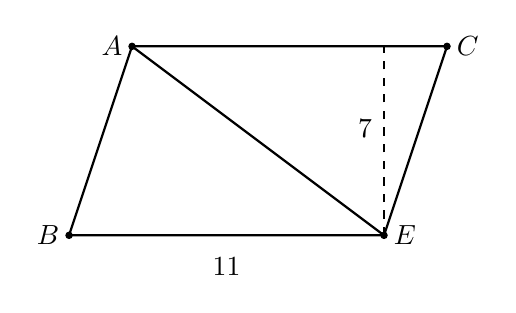
\begin{tikzpicture}[scale=0.8]
  \draw [-, thick] (0,0)--(5,0)--(6,3)--(1,3)--cycle;
  \draw [-, thick] (5,0)--(1,3);
  \draw [-, dashed] (5,0)--(5,3);
  \draw [fill] (0,0) circle [radius=0.05] node[left]{$B$};
  \draw [fill] (5,0) circle [radius=0.05] node[right]{$E$};
  \draw [fill] (6,3) circle [radius=0.05] node[right]{$C$};
  \draw [fill] (1,3) circle [radius=0.05] node[left]{$A$};
  \node at (4.7, 1.7){$7$};
  \node at (2.5, -0.5){11};
\end{tikzpicture}
\end{flushright}

\item The quadrilateral $ABCD$ has a base with length $AB=23$. The area of $\triangle ABC$ is 155.25. Find the height of $ABCD$, the length $h$ of the perpendicular dropped from vertex $C$ to base $\overline{AB}$.\\[0.5cm]
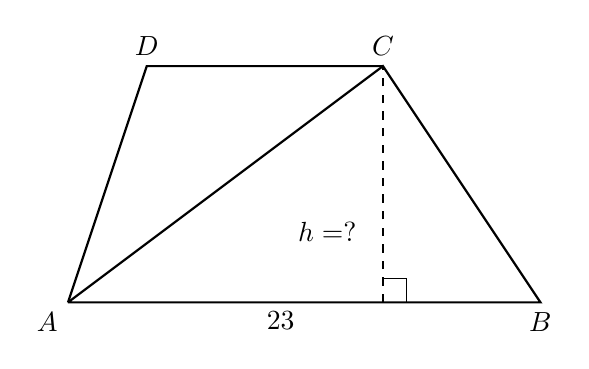
\begin{tikzpicture}[scale=1]
\draw [thick]
  (2,0)node[below left]{$A$}--
  (8,0)node[below]{$B$}--
  (6,3)node[above]{$C$} --(2,0);
  \draw [thick] (2,0)--(3,3)node[above]{$D$} --(6,3);
\draw [dashed] (6,0)--(6,3);
\draw (6,0)++(0.3,0)--++(0,0.3)--+(-0.3,0);
\node at (4.8,0.9)[right]{$h=?$};
\node at (5,0)[below left]{$23$};
\end{tikzpicture} \vspace{0.5cm}

\item The trapezoid $ABCD$ has two parallel sides, $\overline{AB} \parallel \overline{CD}$ with lengths $AB=14$ and $CD=17$. The trapezoid's height is $h=10$. Find the areas of $\triangle ABC$ and $\triangle CDA$. Add their areas to find the area of the whole trapezoid. \\[0.25cm]
   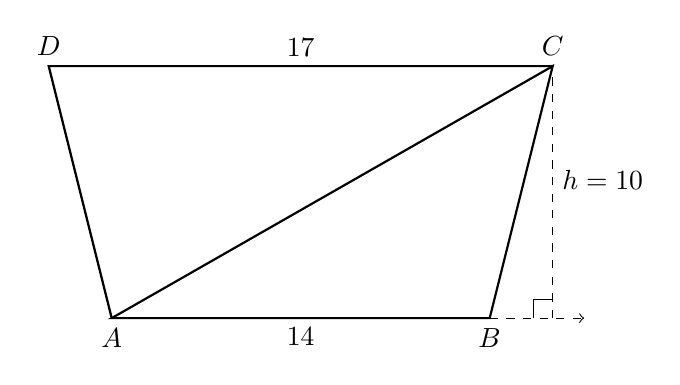
\begin{tikzpicture}[scale=0.8]
    \draw [thick]
       (0,0)node[below]{$A$}--
       (6,0)node[below]{$B$}--
       (7,4)node[above]{$C$} --cycle;
    \draw [thick] (0,0)--(-1,4)node[above]{$D$}--(7,4);
    \draw [dashed] (7,0)--(7,4);
    \draw [dashed, ->] (6,0)--(7.5,0);
    \draw (7,0)++(-0.3,0)--++(0,0.3)--+(0.3,0);
    \node at (7,2.2)[right]{$h=10$};
    \node at (3,0)[below]{$14$};
    \node at (3,4)[above]{$17$};
  \end{tikzpicture} \vspace{1.0cm}
  
\newpage

\item A wooden post laying on the ground is 96 inches long. The post's cross section is square. If its volume is 1152 cubic inches, what is the dimension of each side of its square end, $x$? (not to scale)
\begin{flushright}
  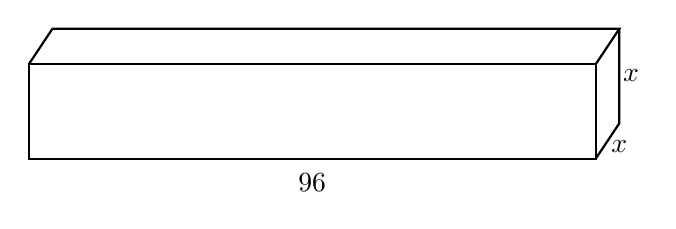
\begin{tikzpicture}[scale=.6]
    \draw [-, thick] (0,0)--(12,0)--(12,2)--(0,2)--cycle;
    \draw [-, thick] (0,2)--(0.5,2.75)--(12.5,2.75)--(12,2);
    \draw [-, thick] (12,0)--(12.5,0.75)--(12.5,2.75);
    \node at (12.75, 1.75){$x$};
    \node at (6, -0.5){$96$};
    \node at (12.5, 0.25){$x$};
  \end{tikzpicture}
  \end{flushright} \vspace{1cm}


\item A rectangle has two triangular cutouts as shown with lengths marked. Find the area of the figure. (the figure is not drawn to scale)
\begin{flushleft}
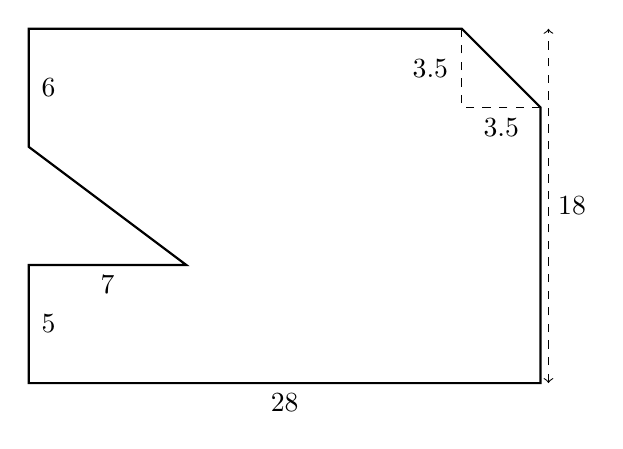
\begin{tikzpicture}[scale=0.5]
  \draw [-, thick] (0,0)--(13,0)--(13,7)--(11,9)--
  (0,9)--(0,6)--(4,3)--(0,3)--cycle;
  \draw [dashed] (13,7)--(11,7)--(11,9);
  \draw [<->, dashed] (13.2,0)--(13.2,9);
  %\draw [fill] (0,0) circle [radius=0.05] node[left]{$A$};
  %\draw [fill] (7,0) circle [radius=0.05] node[right]{$B$};
  %\draw [fill] (7,2) circle [radius=0.05] node[right]{$C$};
  %\draw [fill] (0,2) circle [radius=0.05] node[left]{$D$};
  \node at (0.5, 7.5){6};
  \node at (0.5, 1.5){5};
  \node at (2, 2.5){7};
  \node at (10.2, 8){3.5};
  \node at (12, 6.5){3.5};
  \node at (6.5, -0.5){28};
  \node at (13.8, 4.5){18};
  %\node at (13.5, 8){2};
\end{tikzpicture}
\end{flushleft} \vspace{1cm}

\item Two parallel lines intersect a second set of parallel lines. Given $m\angle1=55^\circ$, find the measures $\angle 2$, $\angle 3$, and $\angle 4$. 
\begin{flushright}
  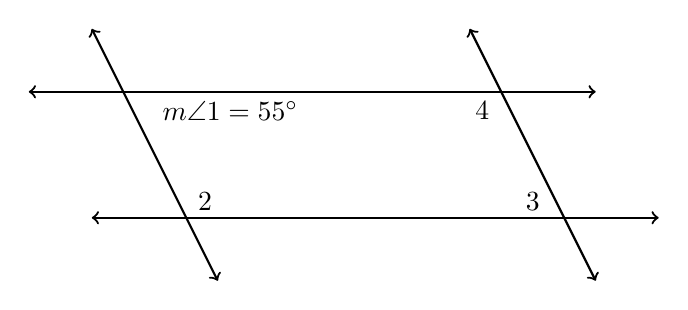
\begin{tikzpicture}[scale=.8]
    \draw [<->, thick] (3,0)--(12,0);
    \draw [<->, thick] (2,2)--(11,2);
    \draw [<->, thick] (5,-1)--(3,3);
    \draw [<->, thick] (11,-1)--(9,3);
    \node at (5.2, 1.7){$m\angle 1 = 55^\circ$};
    \node at (4.8, 0.25){$2$};
    \node at (10, 0.25){$3$};
    \node at (9.2, 1.7){$4$};
  \end{tikzpicture}
  \end{flushright}


  \end{enumerate}
\end{document}
